%% LyX 2.0.4 created this file.  For more info, see http://www.lyx.org/.
%% Do not edit unless you really know what you are doing.
\documentclass[12pt,oneside,english]{amsart}
\usepackage[T1]{fontenc}
\usepackage[latin9]{inputenc}
\usepackage{geometry}
\geometry{verbose,lmargin=1.25in,rmargin=1.25in}
\usepackage{amsthm}
\usepackage{tikz}
\usepackage{array}
\usetikzlibrary{arrows}


\makeatletter
%%%%%%%%%%%%%%%%%%%%%%%%%%%%%% Textclass specific LaTeX commands.
\numberwithin{equation}{section}
\numberwithin{figure}{section}
\theoremstyle{plain}
\newtheorem{thm}{\protect\theoremname}
  \theoremstyle{definition}
  \newtheorem{defn}[thm]{\protect\definitionname}
  \theoremstyle{plain}
  \newtheorem{lem}[thm]{\protect\lemmaname}

\makeatother

\usepackage{babel}
  \providecommand{\definitionname}{Definition}
  \providecommand{\lemmaname}{Lemma}
\providecommand{\theoremname}{Theorem}

\begin{document}

\title{Survey On Online Bipartite Matching and Its Variants}
\author{Caelan Garrett (caelan@mit.edu)}
\author{ Chris Graves (graves@mit.edu)}
\author{Casey O'Brien (cmobrien@mit.edu)}


\maketitle

\section{Introduction}

Although first introduced in 1990 by Karp, Vazirani, and Vazirani
\cite{key-1}, the online bipartite matching problem has in recent
years garnered a lot of new interest due to its applications in Internet
advertising. Like its offline counterpart, the general goal of the
online bipartite matching problem and its variants is to produce an
optimal matching between two mutually exclusive sets of vertices.
Unlike its offline counterpart, however, one of the sets of vertices
is receive online, i.e. one-by-one. On each online step, a vertex
of the online set is given along with its set of adjacent vertices
and the algorithm is tasked with irreversibly matching the incoming
vertex if possible. Variants of this problem include adding weights
on matched vertices and adding uncertainty if a matching will succeed.
These variants generalize the original problem to a wide variety of
applications particuarlly in the domain of online advertising.


\subsection{Organization of the Report}

In Section 2, we will demonstrate and analyze two algorithms (one
deterministic and one random) that solve the classic version of the
online bipartite matching problem. Next, in Section 3, we will present
the online vertex-weighted bipartite matching problem and the analogous
algorithms that solve that problem. Finally, in Section 4 we will
introduce online bipartite matching with stochastic rewards presenting
again both deterministic and random solutions.


\subsection{Preliminaries}

We will begin by formalizing the classic online bipartite matching
problem and providing definitions of some terms which we will use
throughout this paper.


\subsubsection{Classic Online Bipartite Matching Problem Definition}
\label{section:classic}

In the classic version of the problem, as first introduced in \cite{key-1},
we define the input as the bipartite graph $G=(U,V,E)$, where $U$
and $V$ are two independent sets of $n$ vertices each and $E$ is
the set of edges connecting the vertices in $U$ to the vertices in
$V$. For this problem we assume that our algorithm has full access
to all of the vertices in $V$ from the beginning, but receives each
vertex $u\in U$ one at a time in a preselected order. Each time a
vertex $u\in U$ is received, the edges incident to $u$ become known
to the algorithm and the algorithm is thus tasked with permanently
matching $u$ to an adjacent, unmatched vertex $v\in V$ if possible.
The goal of the problem is t o create the largest sized matching possible.
Unless otherwise stated, we assume that $G$ has a perfect matching
and thus the size of the optimal matching is $n$.


\subsubsection{Useful Definitions}
\begin{defn}
We let $N(u)\subset V$ to be the set of previously unmatched vertices
in $V$ that are adjacent to a vertex $u\in U$.
\end{defn}
Thus, it is not until the algorithm receives a vertex $u\in U$ that
the set of vertices $N(u)$ becomes known.
\begin{defn}
We define $m$ as the algorithms current matching and $m(u)$ as the
vertex $v\in V$ that $u$ is matched with. Furthermore, we define
$m^{*}$ as an optimal matching, which we assume is a perfect matching.
\end{defn}

\section{Classic Online Bipartite Matching Algorithms}

Below we present and analyze two algorithms for the classic online
bipartite matching problem (the Greedy algorithm and the Ranking algorithm)
as they were presented in \cite{key-1} and \cite{key-2}.


\subsection{Greedy Algorithm}

The Greedy algorithm, despite its simplicity and na�vet�, actually
provides a reasonable competitiveness, which, as we will later prove,
is optimal for deternministic algorithms.


\subsubsection{Greedy Algorithm Description}

As one might expect, upon reception of a vertex $u\in U$ the Greedy
algorithm works by always, simply matching $u$ with an arbitrary
vertex $v\in N(u)$ if $N(u)\ne\emptyset$. 


\subsubsection{Greedy Algorithm Analysis}

It is easy to see that the Greedy algorithm has a competitive ratio
of at least $\frac{1}{2}$, because for every vertex $u$ it is either
the case that $u$ is matched to some vertex $v\in V$ or $N(u)=\emptyset$.
Remember, we assume that there exists a perfect matching $m^{*}$
which matches all $2n$ of the vertices in $n$ matchings. For every
vertex $u\in U$, at least one of $u$ or $m^{*}(u)$ must be in our
Greedy algorithm's matching. Thus, our algorithm matches a minimum
of $n$ vertices in total in a minimum of $\frac{n}{2}$ matchings. 


\subsubsection{Greedy Algorithm Optimality}

We can further demonstrate that no deterministic algorithm can have
better competitiveness than $\frac{1}{2}$. Suppose, for example,
an adversarial input in which each of the first $\frac{n}{2}$ vertices
from $U$ that the algorithm receives are adjacent to every vertex
$V$. Then the remaining $\frac{n}{2}$ vertices from $U$ are only
adjacent to the vertices that the algorithm was determined to have
had already matched. Thus, clearly for every deterministic algorithm
there is an input for which it is $\frac{1}{2}$ competitive.


\subsection{Ranking Algorithm}

Since the upperbound for the competitiveness of determinstic algorithms
is $\frac{1}{2}$, we will need to add randomization in order to get
an improvement. Luckily, as suggested in \cite{key-1}, by simply
adding a single element of randomness and tweaking our Greedy algorithm
so that there is no arbitrary choice, we can get an improved expected
competitiveness. 


\subsubsection{Ranking Algorithm Description}

The Ranking algorithm begins with an initialization phase that consists
of choosing a random permutation of the vertices in $V$, which will
serve as the basis for our ranking function $\sigma$. Then upon receiving
each vertex $u\in U$, the algorithm matches $u$ to the vertex $v\in N(u)$
which minimizes $\sigma(v)$, such that $v$ has not already been
matched. Obviously, if every vertex adjacent to $u$ is already matched,
i.e. $N(u)=\emptyset$, the algorithm does not match $u$.


\subsubsection{Ranking Algorithm Analysis}
\label{section:ranking analysis}

Like in the Greedy algorithm, a received vertex $u\in U$ is not matched
if and only if $N(u)=\emptyset$. As a result, we know that its competitiveness
is always at least $\frac{1}{2}$. Since, the Ranking algorithm has
a random element to it, it is not bounded in the same way that deterministic
algorithms are, which leads us to the following theorem.
\begin{thm}
The Ranking algorithm has an expected competitiveness of $1-\frac{1}{e}\approx0.63$.
\end{thm}
We will ``prove'' this theorem with an extremely intuitive, but
slightly incorrect proof that is presented in \cite{key-2} for the
sake of intuition. We encourage enthusiastic readers to read \cite{key-2}
in its entirety, if they would like to also get the correct, but more
technical version of the proof. It is important to note here, that
the original proof, as presented in \cite{key-1} had an error that
was detected by Krohn and Varadarajan in 2007. The error was first
corrected by \cite{key-19}, but then quickly simplified in \cite{key-2}.

Let us define $m_{\sigma}$ as the matching produced by the Ranking
algorithm with ranking function $\sigma$ for some given input. We
can relate Ranking($\sigma$) with the optimal matching $m^{*}$ using
the following lemma.
\begin{lem}
\label{lem:For-every-vertex}For every vertex $u\in U$, if vertex
$v=m^{*}(u)$ is not matched in $m_{\sigma}$, then in $m_{\sigma}$
$u$ is matched to a vertex $v'=m_{\sigma}(u)$ such that $\sigma(v')<\sigma(v)$.\end{lem}
\begin{proof}
Since vertex $v$ is not matched in $m_{\sigma}$, that means that
when $u$ was recieved by the Ranking algorithm, $v$ was still unmatched.
Thus, the only reason $u$ would not be matched to $v$ would be if
it could get matched to a higher ranking vertex $v'$, such that $\sigma(v')<\sigma(v)$.
\end{proof}
We will use the following lemma to get our competitiveness.
\begin{lem}
\label{lem:If-we-define}If we define $x_{t}$ as the probability
over ranking function $\sigma$ that the vertex $v\in V$ such that
$\sigma(v)=t$ is matched in $m_{\sigma}$, then $1-x_{t}\le\frac{1}{n}\underset{1\le s\le t}{\sum}x_{s}$
for all $t$ in range $[1,n]$.\end{lem}
\begin{proof}
Let us define $u$ as the vertex in $U$ that $v$ is matched with
in the optimal matching, i.e. such that $v=m^{*}(u)$. Furthermore,
let us define the set of vertices $R_{t-1}\subset U$ as the set of
vertices in $U$ that are matched in $m_{\sigma}$ to vertices in
$V$ of rank that is no more than $t-1$. In otherwords for all $u\in U$
such that $u$ is matched in $m_{\sigma}$, $u$ is in $R_{t}$ if
and only if $\sigma(m_{\sigma}(u))<t$. By Lemma \ref{lem:For-every-vertex},
if vertex $v$ is not matched in $m_{\sigma}$, then $u\in R_{t}$.
Thus, the probability that $v$ is not matched in $m_{\sigma}$ is
bounded by the probability that $u\in R_{t}$. Clearly, by the defintion
of $x_{t}$, the probability that $v$ is not matched is $1-x_{t}$
and the expected size of $R_{t}=\underset{1\le s<t}{\sum}x_{s}$.
If $u$ and $R_{t}$ were independent, then the probability that $u\in R_{t}$
would simply be $\frac{|R_{t}|}{n}=\frac{1}{n}\underset{1\le s<t}{\sum}x_{s}$,
which would complete our lemma with $1-x_{t}\le\frac{1}{n}\underset{1\le s<t}{\sum}x_{s}\le\frac{1}{n}\underset{1\le s\le t}{\sum}x_{s}$
.

However, this is where this proof fails. The fact is $u$ and $R_{t}$
are not actually independent in the way we set it up. The correct,
but less intuitive, proof demonstrates how choosing vertices $v$
and $u$ randomly and independently of $\sigma$ can result in having
the relation that if vertex $v$ is not matched in $m_{\sigma}$,
then $u\in R_{t+1}$. In this case $u$ and $R_{t+1}$ are independent,
which correctly proves the lemma. Again, we encourage interested readers
to read the correct proof in \cite{key-2}.
\end{proof}
Now we can compute the expected competetiveness. It is easy to see
that the expected size of $m_{\sigma}$ is $\sum_{1\le s\le t}x_{s}$.
Since we are assuming that there exists a perfect matching, that means
the expected competitiveness is $\frac{1}{n}\sum_{1\le s\le n}x_{s}$,
which we must lower bound using Lemma \ref{lem:If-we-define}. If
we define $S_{t}=\sum_{1\le s\le t}x_{s}$, we can rewrite Lemma \ref{lem:If-we-define}
to $1-(S_{t}-S_{t-1})\le\frac{1}{n}S_{t}$, which can be simplified
to $1+S_{t-1}\le\left(\frac{n+1}{n}\right)S_{t}$. It follows that
$S_{t}$, and by extension also $\frac{1}{n}\sum_{1\le s\le t}x_{s}$,
is smallest when all of the inequalites are equalities, which gives
us $S_{t}=\sum_{1\le s\le t}\left(\frac{n}{n+1}\right)^{s}$. As a
result, our expected competitiveness $\frac{1}{n}\sum_{1\le s\le n}x_{s}=\frac{S_{n}}{n}$
is lower bounded by $\frac{1}{n}\sum_{1\le s\le n}\left(\frac{n}{n+1}\right)^{s}$
which after some mathemagic becomes $1-(\frac{n}{n+1})^{n}$ which
approaches $1-\frac{1}{e}$ as $n$ goes to infinity, thus concluding
our proof.


\subsubsection{Optimality of Ranking Algorithm}

Now that we demonstrated that the expected competitiveness of the
Ranking algorithm is at least $1-\frac{1}{e}$, the question becomes,
``Is it possible do better?'' The following theorem proven in \cite{key-1},
suggest that no, it is not possible.
\begin{thm}
The competitivess of any online bipartite matching algorithm is bounded
above by $(1-\frac{1}{e})+O(1)$.
\end{thm}
In \cite{key-1}, the authors demonstrate this theorem by proving
that no online algorithm can do better for a particular graph with
exactly one perfect matching in which the first few vertices incoming
vertices from $U$ are adjacent to all or most of the the vertices
in $V$, but the last few vertices from $U$ are only adjacent to
a few or just one of the vertices in $V$. The reason it causes this
bound, after some nontrivial mathematical massaging, is that the first
vertices received from $U$ have many potential vertices to be matched
with from $V$. Thus, it is unlikely that they will be matched with
their optimal matches, which uses up the few potential matches for
the later incoming vertices from $U$ before the algorithm gets to
them.

\section{Online Vertex-Weighted Bipartite Matching}

The online vertex-weighted bipartite matching problem is a generalization of the online bipartite matching problem. The difference is that each vertex in $V$ now has an associated weight. Instead of maximizing the size of the matching, we now aim to maximize the total weight of the vertices of $V$ which are included in the matching. The classic online bipartite matching problem described in Section \ref{section:classic} is the special case where all edges in $V$ have weight 1.

Formally, the input to the problem is a bipartite graph $G = (U, V, E, \{w_v\}_{v \in V})$. The vertices in $V$ as well as their weights are known ahead of time. The vertices in $U$ arrive online. As before, the edges of a vertex $u \in U$ are revealed when $u$ arrives. When a vertex arrives it can either be matched to a neighbor in $V$ or not matched. However, once made, a decision cannot be undone. We aim to maximize the sum of weights of all the matched vertices in $V$. As before, we will assume that $|U| = |V|=n$ and that $G$ contains a perfect matching.

\subsection{Greedy Algorithm}

The obvious greedy solution to this problem is to match a vertex $u \in U$ to its neighbor of greatest weight, or leave it unmatched if it has no remaining neighbors. Call this algorithm $\textsc{Greedy}$.

\begin{lem}
\textsc{Greedy} is a (1/2)-approximation for vertex-weighted bipartite matching. Furthermore, this is the best approximation ratio the algorithm can achieve.
\end{lem}

\begin{proof}
First we show that \textsc{Greedy} is a (1/2)-approximation. Let $O \subseteq E$ be the optimal offline matching, and $A \subseteq E$ be the matching produced by $\textsc{Greedy}$. If $A \neq O$, then there is some $v_{O} \in V$ such that $v_{O}$ is in $O$ but not $A$. Let $u$ be the vertex which was matched to $v_{O}$ in $O$. Then there must be some other vertex $v_{A}$ such that $u$ was matched to $v_{A}$ in $A$. This is because we know that $v_O$ was unmatched when $u$ was being matched, so the only way $u$ would not be matched to $v_O$ is if there were some other neighbor with greater weight.

But now we have that the optimal value `lost' by $u$ is at most equal to the weight of its match in $A$. Therefore the total amount which $A$ `loses' is $|A|$. Hence, $|A| \geq |O|/2$.

To see that this is the tightest approximation ratio for this algorithm, we offer an example. Consider the following graph.

\begin{center}
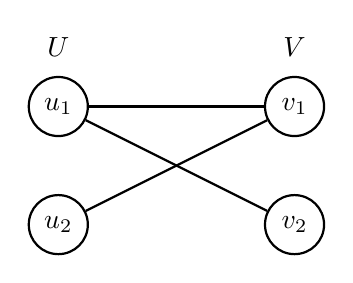
\begin{tikzpicture}[-,>=stealth',auto,
  thick,main node/.style={circle,draw, minimum size = 0.75cm}]

\node[draw = white] (a) at (0, 2.25){$U$};
\node[draw = white] (b) at (3, 2.25){$V$};

\node[main node] (v) at (0, 1.5){$u_1$};
\node[main node] (w) at (0, 0){$u_2$};

\node[main node] (v1) at (3, 1.5){$v_1$};
\node[main node] (w1) at (3, 0){$v_2$};

\path[]


(w) edge node [below] {} (v1)
(v) edge node [below] {} (w1)
(v) edge node [below] {} (v1);

\end{tikzpicture}
\end{center}

Say that vertices arrive in the order $(v_1, v_2)$, and let $w_{v_1} = 1 + \epsilon$ for some $\epsilon > 0$ and $w_{v_2} = 1$. Then the greedy algorithm will match only $(u_1, v_1)$, and the optimal solution will match $(u_1, v_2), (u_2, v_1)$. As $\epsilon$ approaches 0, the approximation ratio approaches $1/2$.

\end{proof}

We will not offer a proof here, but it turns out that here, as in the case with equal weights, no deterministic algorithm can do better than $\textsc{Greedy}$.

\subsection{Generalizing Ranking}

Consider the \textsc{Ranking} algorithm described above. For an input in which the range of weights is small, this algorithm will perform well. This is reflected in the fact that \textsc{Ranking} is optimal in the case where all weights are equal. However, when the range of weights is large, this algorithm can perform very poorly.

We want to generalize the ranking algorithm in order to account for the weighted case. We will present a new algorithm which we will call \textsc{Perturbed-Greedy}, and then we will show that this algorithm is equivalent to \textsc{Ranking} in the case where all weights are equal.

The \textsc{Perturbed-Greedy} algorithm will use the function
\[\psi(x) = 1 - e^{x - 1}.\]

\begin{enumerate}
\item For each $v \in V$, choose $x$ uniformly at random from $[0, 1]$.
\item For arriving $u \in U$, match $u$ to the unmatched neighbor $v$ with highest value $b_v\psi(x)$.
\item Break ties by vertex ID.
\end{enumerate}

Consider the case where all weights are equal. Since $x$ is chosen uniformly at random, choosing vertices according to the highest values of $b_v\psi(x)$ is equivalent to choosing a random ranking. Thus, \textsc{Perturbed-Greedy} is equivalent to \textsc{Ranking} when all weights are equal, as desired.

\begin{thm}
\textsc{Perturbed-Greedy} achieves an approximation ratio of $1 - \frac{1}{e}$ for the vertex-weighted online bipartite matching problem.
\end{thm}

We will not offer a proof of this theorem here. However we note that this is consistent with the approximation of \textsc{Ranking}. It turns out that, as is the case with \textsc{Ranking}, this is the optimal approximation ratio for this problem. Intuitively, this result seems reasonable because we know that this is the optimal approximation ratio for the more specific version of this problem.

The proof of the approximation ratio of \textsc{Perturbed-Greedy} is quite similar to the proof of the approximation ratio of \textsc{Ranking} in Section ~\ref{section:ranking analysis}. We encourage readers to read this proof, as well as the proof of the optimality of the approximation ratio, in [[[[[]]]].

\section{Stochastic Online Bipartite Matching}

\subsection{Stochatic Variant Definition}Another interesting variant of the online bipartite matching problem is online bipartite matching with stochastic rewards \cite{key-4}. The setup is similar to the classic problem \cite{key-1} where the goal is to maximize the number of matchings between a stream of vertices $V$ and with known vertices $U$. The twist is that each matching has some probability of success $p_{uv}$. The goal is now to maximize the expected number of successful matchings given that some may fail. The variant of this problem was motivated by its practical applications to internet advertising and crowdsourcing. Internet advertising involves matching advertisers' ads to be shown to users of a service where advertisers pay each time a user clicks on an ad (pay-per-click advertising). The likelihood that a user $u$ clicks on an ad $v$ can be modeled by a probability $p_{uv}$. Thus, this matching problem can be modeled as an online stochastic reward matching problem where the service wants to maximize its revenue given a stream of ads to be matched with users. This setup can also model crowdsourcing where each worker $u$ has a probability $p_{uv}$ of completing task $v$ so the online assignment hopes to maximize the expected number of completed tasks. 

Solving this problem for arbitrary $p_uv$ is an open problem, however, Mehta and Panigrahi present online algorithms and analysis for the problem when $\forall{u,v}: p_{uv} = p$. These algorithms and their bounds on competitive ratios can still be practically usable for the above applications if the variance in $ p_{uv}$ is small. For example in online advertising, the probability of a user clicking on an ad is small for almost all users so using one estimate for $p$ should still give informative, approximate bounds. Additionally, the case where $p \rightarrow 0$ (called a vanishing probability) is interesting theoretically on its own. 

\subsection{Optimal Algorithm}As with any online algorithm problem, algorithms are compared to an optimal algorithm that knows the input stream (the full bipartite graph). A complication here is the non-determinism of the matching success. To mend this, the optimal algorithm (\textsc{OPT}) is defined non-stochastically as being able to fractionally match vertices to maximize $\sum_u{\sum_v{p x_{uv}}}$ such that $\sum_u{x_{uv}} \leq 1$. By giving \textsc{OPT} more power, it upper bounds the best matching of any algorithm. Note that for most graphs, the expected number of matchings is $p |U| = p n$ which is used to simply the analysis.

\subsection{Adaptive versus Non-Adaptive}Algorithms for this problem are separated into two categories: adaptive and non-adaptive. After each pair is matched, the match's success is immediately computed according to $p$. If successful, u and v are both removed from the set of unmatched vertices and the match is scored. Otherwise, u is removed from the set of unmatched vertices, and v remains free to be matched later. An adaptive algorithm can learn the result of a matching immediately and attempt to rematch v with a later u if prior matches failed. However, a non-adaptive algorithm does not learn this information until after the algorithm completes and may try to rematch a v that was already successfully matched. In this case, only 1 successful matching is scored for each v. Intuitively, non-adaptive algorithm are less powerful than adaptive algorithms because they learn less information which results in a lower expected score. In fact, it can be proven that the competitive ratio of non-adaptive algorithms for this problem is at most $1/2$ when $p \rightarrow 0$ by applying Yao's minimax principle on a particularly bad distribution of inputs for a deterministic algorithm. This then bounds the best performance of any randomized algorithm. The proof isn't fully presented in the paper and isn't that interesting.

As expected, adaptive algorithms have more power than non-adaptive algorithms and are able to achieve better competitive ratios. An extension of \textsc{Ranking} seen earlier performs well when $p \rightarrow 1$ giving the same competitive ratio as the non-stochastic classic problem. But interestingly enough, a deterministic algorithm called \textsc{Stochastic Balance} performs better when $p \rightarrow 0$. And this algorithm's competitive ratio is $1/2$ when $p = 1$ showing that it is consistent with the theorem that any deterministic algorithm has competitive ratio of at most $1/2$ in the classic problem.

\subsection{Proof Techniques}Before diving into these algorithms, we note a generalization of the stochastic bipartite matching problem that makes analysis of these algorithms possible.
Stochastic matching can be viewed as a packing problem where each $v$ has (prior to running any algorithm) a randomly choosing bin size which represents the number of matches that must be made before that vertex will have a successful match. More specifically, this threshold is a geometric random variable given by the following.

\begin{defn}$Pr[\theta_u = pt] = p(1-p)^{t-1}$
\end{defn}

In this generalization, the goal is to maximize the expected number of filled bins such that these bins have had enough potential matches that one of them now succeeded. Note however that adaptive algorithms working under this view don't know the size of each bin until it is filled which is consistent with learning the success of a matching. More generally this equating of load on a bin with probability of a successful match can be proven by a simply argument from linearity of expectation. 

The competitive ratio of both of these algorithms is proved using a technique called factor-revealing linear programming \cite{key-5}. Drawing from ideas involving the duality between the algorithm and an adversary, it formulates the adversary's "choice" of some outcomes of the algorithm to maximize the number of vertices that are not matched. The adversary's moves however are constrained to be consistent with the applied algorithm. After finding this primal linear program, taking the dual and applying weak duality to some feasible solution of the dual gives an upper bound on the maximum primal objective value. Thus, the result is an upper bound of the worst possible performance of the algorithm giving the bound on the competitive ratio. The goal of the algorithmist is to find a set of constraints that follow from running the algorithm that limit the ability of the adversary to maximize the worst case performance. This technique is particularly effective because of the algorithms' simplicity allows them to be encoded into these constraints. 

\subsection{Ranking Algorithm}\textsc{Ranking} is the same as previously presented with the ability to adaptively rematched failed matchings. \textsc{Ranking} randomly permutes the set of U vertices. Upon an incoming vertex to be matched, the algorithm matches it with the highest ranked neighbor that has not been successfully matched. The analysis introduces the notion of a good matching and a bad matching. A bad matching occurs when matched edge $(u, v)$ has $rank(u) < rank(opt(v))$ . The intuition is that the algorithm matched a vertex too early (earlier than the optimal). Otherwise, the matching is a good match. $good(s)$ and $bad(s)$ are respectfully defined to be the expected load of the vertex $u$ with $s = rank(u)$ due to good matches and bad matches. The linear program takes the following form where the adversary chooses $good(s)$ and $bad(s)$ to minimize the expected number of matches under some algorithmic constraints. 

\begin{defn} \textsc{Ranking} Factor-Revealing Linear Program \\
minimize $\sum_{s}{match(s)}$ \\
subject to \\
$1) \forall{s}: match(s) = good(s) + bad(s)$\\
$2) \forall{t}: \frac{1 - (1-p)^{\frac{1}{p}}}{p} - match(t) \leq \sum_{s \leq t}{\frac{bad(s)}{n-s}}$ \\
$3) \forall{t}: \sum_{s \leq t}{\frac{s*bad(s)}{n-s}} \leq \sum_{s \leq t + 1}{good(s)}$ \\
$4) \sum_{t}{match(t)} \geq \frac{1}{2} + \frac{\sum_{t}{good(t)}}{2}$
\end{defn}

Constraint 1) trivially comes from the definitions of $good(s)$ and $bad(s)$. The other constraints are more involved. We prove only Constraint 2) to give the flavor for how these are discovered. The proof of the Constraint 3) is found in \cite{key-19}.

\begin{lem} Constraint 2)
\begin{proof} Recall that using our bin load approach, we defined a vertex $u$ being successfully matched if its load equaled $\theta_u = match(rank(u))$ here. So if the vertex at rank $t$ is matched on expectation $E[\theta_u] = \frac{1 - (1-p)^{1/p}}{p} = match(t)$ and $ \frac{1 - (1-p)^{1/p}}{p} - match(t) = 0$ satisfying the constraint. Otherwise if rank $t$ is not matched on expectation, we know that incoming $v$ vertices that would have been matched to $u$ by \textsc{OPT} must be matched to some $u'$ with a smaller rank. It follows that this set of $v$ vertices contains at least the missing load from the vertex at rank $t$ giving the set load at least $\frac{1 - (1-p)^{1/p}}{p} - match(t)$. Now we look for an upper bound on the load of this set. We notice that the mismatch of these $v$ vertices constitutes a bad matching for each position $s$ they are matched because for some permutations of the ranking order they matched the vertex differently than  \textsc{OPT}. Furthermore, it would have been a bad matching for any of the $n-s$ permutations if $u$ had been later in ranking than $s$. So the permutation with $u$ at $t$ is expected to give $\frac{1}{n-s}$ of the bad match load of $s$. Thus the upperbound on this load is $\sum_{s \leq t}{\frac{bad(s)}{n-s}}$ giving the constraint.
\end{proof}
\end{lem}

\begin{thm} Competitive Ratio for \textsc{Ranking} is $((1-\frac{1}{e}) - (1-\frac{1}{e})(1-p)^{1/p})$
\begin{proof}
Upon taking the dual of this linear program and finding a feasible solution to the dual, the authors indicated that their solution had objective function lower bounded by $((1-\frac{1}{e}) - (1-\frac{1}{e})(1-p)^{1/p})(\frac{n}{p})$ which in turn bounds the worst performance of the adversary giving a competitive ratio of $((1-\frac{1}{e}) - (1-\frac{1}{e})(1-p)^{1/p})$
\end{proof}
\end{thm}

\subsection{Stochastic Balance Algorithm}\textsc{Stochastic Balance} algorithm doesn't involve any randomization. Instead, it records the load of each $U$ (which as mentioned is the number of failed matches $* p$) and an incoming vertex to the neighbor with the least load that is also not successfully matched. The analysis for this algorithm uses the same factor-revealing linear programming approach but with a different language for constraining the adversary. It defines $f_u(x)$ to be the variables of the linear program corresponding to the probability that vertex $u$ has failed to be matched at the end of the algorithm with load $x$. Note that the number of load levels is linear with $|V|$ because there are at most $|V|$ matching edges to any $u$ which contribute $p$ to the load. Thus the expected number of failures for the algorithm is $\sum_{u}{\sum_{x}f_u(x)}$ which the adversary attempts to maximize under constraints of \textsc{Stochastic Balance}. Finally, $L^*_u$ is an additional variable encoding the load assigned to $u$ by \textsc{OPT}.

\begin{defn} \textsc{Stochastic Balance} Factor-Revealing Linear Program \\
maximize $\sum_{u}{\sum_{x}f_u(x)}$ \\
subject to \\
$1) \forall{x}: \sum_{y \leq x}{\sum_u{(1+L^*_u)f_u(y)}} + (1-p)^{x/p}\sum_{y>x}{(1-p)^{-y/p}(\sum_u{f_y(y)})} \leq n$ \\
$2) \forall{x}: \sum_u{((1-p)^{-L^*_u/p} + \sum_{y<L^*_u}{f_u(y)(1 + L^*_u - x)(1-p)^{-y/p})}} \leq n$\\
$3) \sum_x{\sum_u{f_u(x)(1-p)^{-x/p}}} = n $
\end{defn}

Like in \textsc{Ranking} analysis, we prove Constraint 1) to show the flavor for how these are constructed and along the way prove Constraint 3). The original paper itself only sketches out the proof of the Constraint 2) \cite{key-4}.

\begin{defn}Let $L^{\infty}_u(\theta)$ be the load on vertex $u$ given that $\theta$ is modified such that $\theta_u = \infty$ or in words the load on $u$ when the algorithm finishes under the other vertices thresholds. 
\end{defn}

\begin{defn}
Let $q_u(x) = \sum_{\theta: L^{\infty}_u(\theta)=x}{Pr[\theta = \theta_{-u}]}$ This just encodes the probability that $x$ is an resulting load for $u$ as sum of the individual likelihoods of drawings of $\theta$. 
\end{defn}

\begin{lem} $f_u(x) = (1-p)^{(x/p)}q_u(x)$ 
\begin{proof}
$f_u(x) = Pr[(\theta_u > x) \wedge (L^{\infty}_u(\theta_{-u}) = x)]$ \\
$f_u(x) = Pr[\theta_u > x]Pr[L^{\infty}_u(\theta_{-u}) = x]$ \\
$f_u(x) = (1-p)^{(x/p)}q_u(x)$ 

This follows from representing the probability of a resulting load being unsuccessful as the intersection of when the load is less than its threshold and the result of the vector constitutes an unsuccessful load vector. By independence, this separates giving the resulting expression where $(1-p)^{(x/p)}$ indicates that the matching fails $x/p$ times, and $q_u(x)$ is an unsuccessful resulting load. We can represent the probability that a load $x$ succeeds for vertex $u$ as $g_u(x)$ and find a similar looking expression. 
\end{proof}
\end{lem}

\begin{lem} $g_u(x) = p(1-p)^{(x/p-1)}\sum_{y \geq x}{q_u(y)}$ 
\begin{proof}
$g_u(x) = Pr[(\theta_u = x) \wedge (L^{\infty}_u(\theta_{-u}) \geq x)]$ \\
$g_u(x) = Pr[\theta_u = x]Pr[L^{\infty}_u(\theta_{-u}) \geq x]$ \\
$g_u(x) = p(1-p)^{(x/p-1)}\sum_{y \geq x}{q_u(y)}$ 

This follows from noting that a load is successful if it equals its threshold. But also, the resulting load of the algorithm if there is no limit on the load must give some load greater than $x$ or $x$ is not possible. This probability of the first part is $ p(1-p)^{(x/p-1)}$ while the probability of the second is the sum of each of these disjoint $q_u(y)$ evens. Because $f_u(x)$ and $g_u(x)$ are defined complementarily, we note their sum over the possible loads and vertices must equal the total number of vertices, $\sum_u{\sum_x{(f_u(x) + g_u(x))}} = n$. Substituting $g_u(x)$ for $f_u(x)$ gives Constraint 3)
\end{proof}
\end{lem}

\begin{lem} Constraint 1)
\begin{proof}
$\sum_{y \leq x}{\sum_u{L^*_uf_u(y)}} \leq \sum_{y \leq x}{y \sum_u{(f_u(y) + g_u(y))}} + x\sum_{y > x}{\sum_u{(f_u(y) + g_u(y))}}$ \\
$\sum_{y \leq x}{\sum_u{(1+L^*_u)f_u(y)}} + (1-p)^{x/p}\sum_{y>x}{(1-p)^{-y/p}(\sum_u{f_y(y)})} \\
\leq \sum_x{\sum_u{f_u(x)(1-p)^{-x/p}}} = n$

This is because for a vertex $u$ that ends up with load $x$, all $u'$ on the \textsc{OPT} solution that took a possible matching from $u$ must have had a lower load at the time to be picked before $u$ by the  \textsc{Stochastic Balance}. So the expected sum of optimal loads assigned when the algorithm fails an assignment are less than the sum of expected load of the failed vertices produced by  \textsc{Stochastic Balance}. Substituting $g_u(x)$ for $f_u(x)$, simplifying, and appling the equality learned in Constraint 3) gives Constraint 1).
\end{proof}
\end{lem}

\begin{thm} Competitive Ratio for \textsc{Stochastic Balance} is $(1+(1-p)^ {2/p})/2$
\begin{proof}
Using the weak duality again, the authors mention that a bound on the linear program gives competitive ratio of $(1+(1-p)^ {2/p})/2$. The intersection of these two functions for the competitive ratios of \textsc{Ranking} and \textsc{Stochastic Balance} shows that the latter performs better when $p < 0.26$. Thus unlike the classic and weighted case, a deterministic algorithm is so far been proven to perform better than the randomized algorithm as $p \rightarrow 0$.
\end{proof}
\end{thm}

%Insert image of graphs

\section{Conclusion}

Since the original paper published in 1990, the online bipartite matching problem and its variants have gained a lot of attention, in particular in regards to its applications to online advertising. Through this paper we explored the original online bipartite matching problem, the problem with weighted vertices, and the problem with stochastic rewards. Without offering complete formal proofs, we have presented many of the most important results pertaining to this set of problems.

\section{Acknowledgements}

We would like to thank Professor Karger for a great semester.

\begin{thebibliography}{{[}AGKM{]}}
\bibitem[{[}KVV{]}]{key-1} R. Karp, U. Vazirani, and V. Vazirani,
\textquotedblleft{}An optimal algorithm for online bipartite matching,\textquotedblright{}
in Proceedings of the 22nd Annual ACM Symposium on Theory of Computing,
1990. (http://www.cs.berkeley.edu/\textasciitilde{}vazirani/pubs/online.pdf)

\bibitem[{[}BM{]}]{key-2} B. Birnbaum and C. Mathieu, \textquotedblleft{}Online
bipartite matching made simple,\textquotedblright{} 2008. (http://cs.brown.edu/\textasciitilde{}claire/Publis/sigactnews08.pdf)

\bibitem[{[}GM{]}]{key-19}Gagan Goel and Aranyak Mehta. Online budgeted
matching in random input models with applications to adwords. In SODA
'08: Proceedings of the nineteenth annual ACM-SIAM symposium on discrete
algorithms, pages 982-991, Philadelphia, PA, USA, 2008. Society for
Industrial and Applied Mathematics.

\bibitem[{[}AGKM{]}]{key-3} Gagan Aggarwal, Gagan Goel, Chinmay Karande,
and Aranyak Mehta, \textquotedblleft{}Online vertex-weighted bipartite
matching and single-bid budgeted allocations,\textquotedblright{}
SODA, 2011. (arXiv:1007.1271 {[}cs.DS{]})

\bibitem[{[}MP{]}]{key-4} A. Mehta and D. Panigrahi, \textquotedblleft{}Online
matching with stochastic rewards,\textquotedblright{} FOCS, 2012,
pp. 728-737. (http://www.cs.duke.edu/\textasciitilde{}debmalya/papers/focs12-matching.pdf)

\bibitem[{[}JMMSV{]}]{key-5} K. Jain, M. Mahdian, E. Markakis, A. Saberi, and V. V.
Vazirani, \textquotedblleft{}Greedy facility location algorithms analyzed using
dual fitting with factor-revealing lp,\textquotedblright{} J. ACM, vol. 50, no. 6, pp. 795-824, 2003.

\end{thebibliography}
 

\end{document}
